\chapter{Numerical study}
\label{chap: Std Schwinger Model}

As we mentioned earlier in this paper, the Schwinger model (QED$_2$) is a subject of interest in computational physics since it can lead to a broader understanding of some aspects of QCD$_4$, in particular for what concerns the study of the chiral limit of the theories. 
\\ In our case study we implemented dynamical fermions thanks to the introduction of Wilson fermions, which suffer from an explicit breaking of the chiral $SU(2)_A \times U(1)_A$ symmetries, but we expect the chiral symmetry to be restored at a critical fermion coupling $\kappa_c(\beta).$
\\ In this Chapter, after a brief overview about stochastic estimators typically used in LQCD simulations, the so-called \textit{noise vectors}, we will present some tests conducted on our system in order to investigate more deeply the chiral limit of the Schwinger model.
\\ For instance, the low lying spectrum of the Schwinger model with two mass-degenerate fermions contains an iso-triplet of light particles (which we denote as "pions" $\pi$ by analogy to QCD), which become massless in the chiral limit, and a massive iso-singlet state (the "$\eta$" meson), which leads to a $U(1)$ problem analogous to the one we study in QCD$_4$.\footnote{For $N_f$ massless quarks, QED$_2$ would show one massive and $N_f - 1$ independent massless bosons.}
\\ The first step of our investigation consists in understanding how to reach the chiral limit, i.e. how to fine-tune the bare parameters of our system in order to drive the quark mass (and the pions' mass) to zero. The quark mass $m$ is defined through the implementation of a PCAC relation \cite{Hip_1998}, so that we can study the critical fermion coupling $\kappa_c(\beta)$ at which chiral symmetry is restored, since there is not a simple order parameter which allows us to identify that point in coupling phase space.
\\ Consequently, we focus on the aforementioned low-lying spectrum, retrieving the $\pi$'s and $\eta$ masses from the study of \textit{two point correlation functions}. We compare the results with some simulations in literature \cite{Hip_1998, Gattringer_1999, Christian_2006, https://doi.org/10.48550/arxiv.2201.08008}, as well as for analytical predictions \cite{BELVEDERE1979112, https://doi.org/10.48550/arxiv.hep-th/9505168, Hosotani_1998}.
\\ This tests are useful to pave the way for a future comparison between the standard Schwinger Model simulations and simulations where we embed the fermion determinant factorization we will discuss in the following chapters.


\section{Chiral Condensate and Noise Vectors}
As we stated before, the massive Schwinger Model is an instructive framework, as it shares various non-perturbative features with QCD. For instance, it is embedded with a non-vanishing \textit{chiral condensate}, which for a $L_0 \times L_1 = V$ lattice with $N_f$ quark flavors it is defined as:
\begin{equation}\label{cc}
    \Sigma = - \langle \Bar{\psi} \psi \rangle = - \frac{1}{V} \frac{1}{N_f} \sum_x \sum_{i = 1}^{N_F} \langle \Bar{\psi}_i (x) \psi_i(x) \rangle 
\end{equation}
where $\langle \dots \rangle$ here denotes an expectation value taken over fermionic degrees of freedom and over different gauge configurations. For what concerns the fermionic expectation value, we can use Wick's theorem:
\begin{equation}
    \langle \Bar{\psi}_i(x) \psi_i (x) \rangle_F = \tr(D^{-1}(x,x))
\end{equation}
where $\tr(\dots)$ denotes a trace over the spinorial indices. Hence (\ref{cc}) becomes:
\begin{equation}
    \Sigma = \frac{1}{V} \sum_x \langle \tr D^{-1}(x,x) \rangle = \frac{1}{V} \langle \Tr D^{-1} \rangle
\end{equation}
where $\Tr$ now denotes a trace over both spinorial indices and space-time points.
\\ Lattice gauge calculations of this kind in QCD typically involve an enormous amount of degrees of freedom, even for relatively small lattices: it is non feasible to manage such computations exactly, and there comes the necessity to treat the problem with a stochastic approach. Many suggestions have been proposed to give an approximate solution for matrix inversion algorithms \cite{PhysRevB.34.7911, PhysRevD.32.2736, DONG1992353,BITAR1989348}, and here we will focus on the idea of stochastic estimation with \textit{noise vectors}. In order to invert a matrix of dimensions $L \times L$, we introduce an ensemble of $N_{noise}$ column vectors $\{\eta^{(n)}\}_{n = 1, \dots, N_{noise}}$ with the following orthonormality features:
\begin{equation}\label{noise}
    \langle \eta_i \rangle = 0 \hspace{10mm} \langle \eta_i \eta_j \rangle = \frac{1}{N_{noise}} \sum_{n = 1}^{N_{noise}} \eta^{(n)}_i \eta^{(n)}_j = \delta_{ij}
\end{equation}
where $\eta_i^{(n)}$ is the $i$-th entry of the $n$-th noise vector. Notice that these properties are strictly true in the limit $L \to \infty$.
Noise vectors allow us to approximate the trace of $D^{-1}$, since:
\begin{equation}\label{Noise trace}
    \Tr D^{-1} \simeq \frac{1}{N_{noise}} \sum_{n = 1}^{N_{noise}} (\eta^{(n)})^\dagger D^{-1} \eta^{(n)}
\end{equation}
Any complete set of vectors which satisfies (\ref{noise}) can be used to estimate the matrix elements of $D^{-1}$. Consider for instance Gaussian noise vectors, hence vectors with probability distribution $P(\eta^{(n)}_i(x)) \sim \exp(-(\eta^{(n)}_i(x))^*(\eta^{(n)}_i(x)))$. If we take the following expectation value on the ensemble of noise vectors:
\begin{equation}
    \langle (\eta^{(n)}_i(x))^*(\eta^{(n)}_j(y)) \rangle = \delta_{ij} \delta_{xy}
\end{equation}
we can show that in the limit of infinite noise vectors $N_{noise} \to \infty$:
\begin{equation}
    \begin{split}
        \lim_{N_{noise} \to \infty} \frac{1}{L} \sum_{n = 1}^{N_{noise}} (\eta^{(n)})^\dagger D^{-1} \eta^{(n)} & = \frac{\int d\eta \, \eta^\dagger_i(x) D^{-1}_{ij}(x,y) \eta_j(y) e^{-\eta^\dagger \eta}}{\int d\eta \, e^{-\eta^\dagger \eta}} = \\ & = D^{-1}_{ij}(x,y)\delta_{ij} \delta_{xy} = \Tr D^{-1} 
    \end{split}
\end{equation}
In our case study, we evaluated the efficiency of different kinds of noise vectors, namely Gaussian vectors, $\mathbb{Z}_2$, $\mathbb{Z}_4$ and $U(1)$ vectors. Gaussian vectors have been drawn with a routine developed by M. Lüscher in \cite{L_scher_1994}, which exploits the so-called Box-Muller algorithm \cite{10.1214/aoms/1177706645}. Given two independent random variables $U_1, U_2$ chosen from the uniform distribution on the unit interval (0, 1], one can show that:
\begin{equation}
    z_0 = \sqrt{-2 \ln(U_1)} \cos(2\pi U_2) \hspace{5 mm} z_1 = \sqrt{-2 \ln(U_1)} \sin(2\pi U_2) 
\end{equation}
are two independent random variables with a standard normal distribution.
\\ For what concerns $\mathbb{Z}_2$ and $\mathbb{Z}_4$, each vector component was randomly drawn respectively between $\{\pm 1\}$ and $\{\pm 1, \pm i\}$, while for $U(1)$ noise vectors each component is simply a complex phase $e^{i\theta}$, with $\theta \in \left[0, 2\pi\right]$.
\\ Consider Eq. (\ref{Noise trace}) again. Since the result would be exact only in the limit of infinite sources, we want to study more in-depth the contributions to the error on the estimate. This kind of measure has two sources of error: the fluctuations of $\Sigma$ from a gauge-configuration to another and the accuracy of the stochastic estimate on each configuration. The first term does not depend on the number of sources we embed in the computation, while the second term should scale as $\sim 1/\sqrt{N_{noise}}$, hence if we take a large number of sources the gauge-contribution will be dominant, and we would not increase the estimate precision by taking a larger ensemble of noise vectors.
\\ As a first test, let's check whether the errors coming from the stochastic estimates follow this behaviour. Given a fixed gauge-configuration, we can compute the expected value of the chiral condensate exactly through the definition \eqref{cc}, since for small lattices it is feasible to compute the trace of the propagator matrix $D^{-1}$.
This computation relies on the introduction of $\textit{point sources}$, but since we will embed this technique heavily in the following chapters, we leave the technical details for later.
\\ On the other hand, we estimated $\Sigma$ with an increasing amount of stochastic sources for each kind of noise vector, repeating each measure multiple times in order to see how the stochastic estimates distributed. Operatively, we simulated a $16 \times 16$ lattice with $\beta = 2.0$ and $m_0 = 0.2$, and for each type of noise vectors we let $N_{noise}$ range between $5$ and $100$, with a step of $5$ sources. Each measure has been replicated $100$ times, and in figures (\ref{fig:cc_g})-(\ref{fig:cc_z4}) we plotted the last estimate for each value of $N_{noise}$, while the error bar $\sigma_\Sigma$ is given by the standard deviation of the distribution, i.e.:
\begin{equation}
\sigma_{\Sigma} = \sqrt{\frac{\sum_{i = 1}^{100} (\Sigma_i - \Bar{\Sigma})^2}{(N-1)}}     
\end{equation}
where $\Bar{\Sigma}$ indicates the exact computation of the chiral condensate, obtained from the trace of the propagator, and its value is represented in each plot through a green horizontal line.
We see that the estimates get roughly closer to the exact computation as the number of sources is increased, and the distribution becomes narrower. For a deeper analysis, we plotted the value of $\sigma_\Sigma$ against $1/\sqrt{N_{noise}}$ in order to verify the expected behaviour for the errors on the estimates and give some insights on the different kinds of noise vectors.
\\ From Figure \ref{fig:noise_errors} we can draw a first conclusion, namely Gaussian vectors lead to bigger errors, hence one would prefer different sources in actual lattice computations.
In Figures (\ref{fig:dev_g})-(\ref{fig:dev_z4}) we depicted more clearly the expected behaviour for $\sigma_\Sigma$, as for each kind of noise vectors the linear relation with respect to $1/\sqrt{N_{noise}}$ is evident. The green lines show a "linear fit", where a Gaussian error is automatically assigned to each point of the datasets, but it should be regarded only as a visual way to guide the eye.
\begin{figure}[H]
\centering
              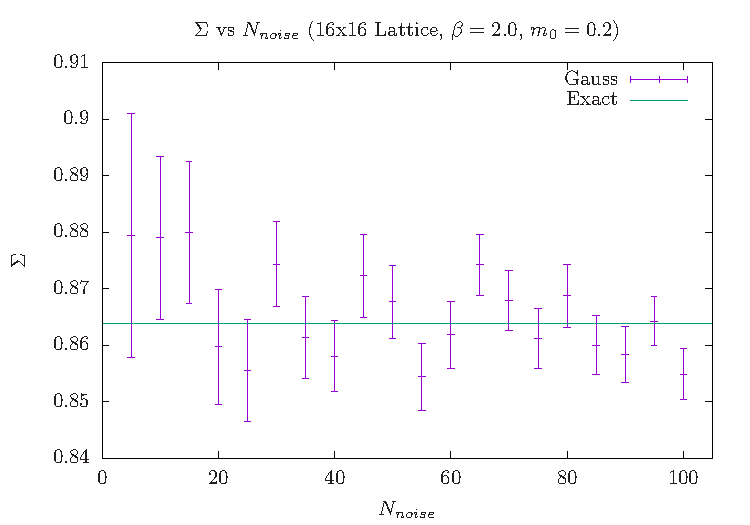
\includegraphics[width=0.8\linewidth]{images/cc_g.pdf}
              \caption{Estimate of $\Sigma$ with Gaussian vectors.}
              \label{fig:cc_g}
\end{figure}
\begin{figure}[H]
\centering
              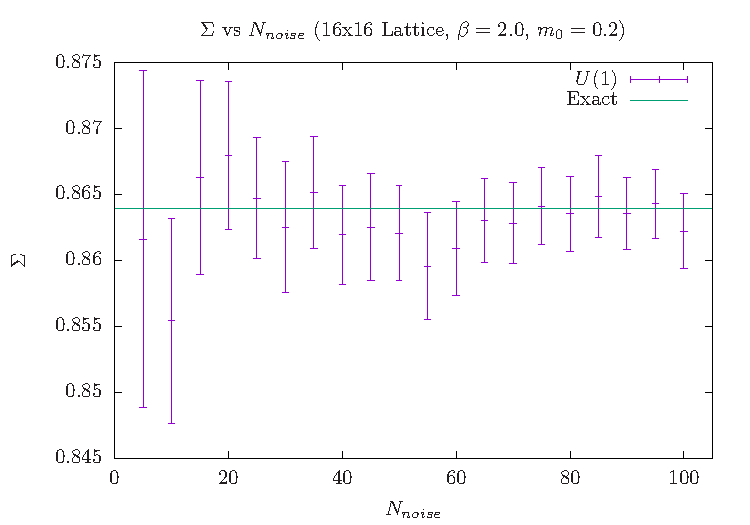
\includegraphics[width=0.8\linewidth]{images/cc_u1.pdf}
              \caption{Estimate of $\Sigma$ with $U(1)$ vectors.}
              \label{fig:cc_u1}
\end{figure}
\newpage
\begin{figure}[H]
\centering
              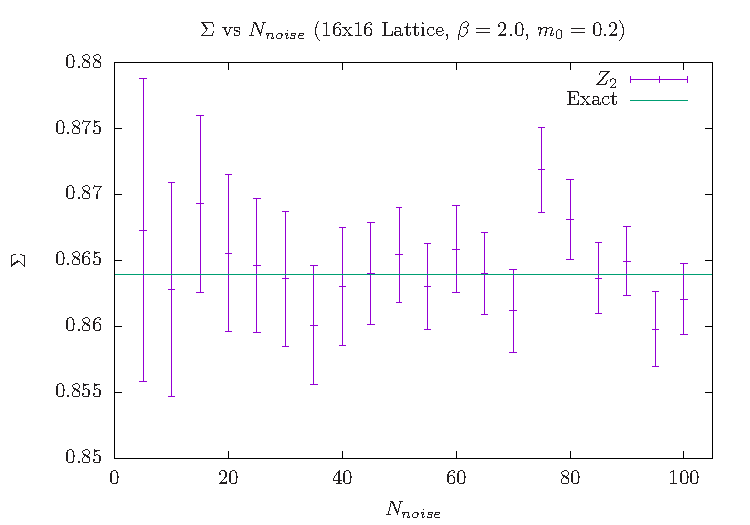
\includegraphics[width=0.8\linewidth]{images/cc_z2.pdf}
              \caption{Estimate of $\Sigma$ with $\mathbb{Z}_2$ vectors.}
              \label{fig:cc_z2}
\end{figure}
\begin{figure}[H]
\centering
              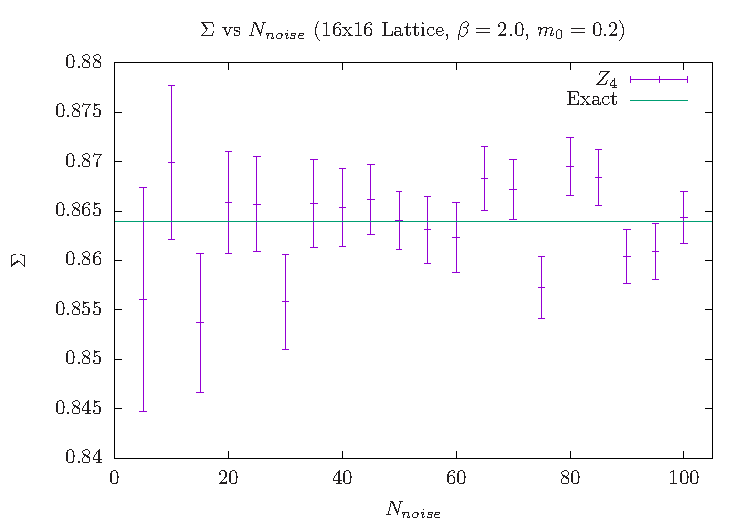
\includegraphics[width=0.8\linewidth]{images/cc_z4.pdf}
              \caption{Estimate of $\Sigma$ with $\mathbb{Z}_4$ vectors.}
              \label{fig:cc_z4}
\end{figure}
\begin{figure}[H]
    \centering
    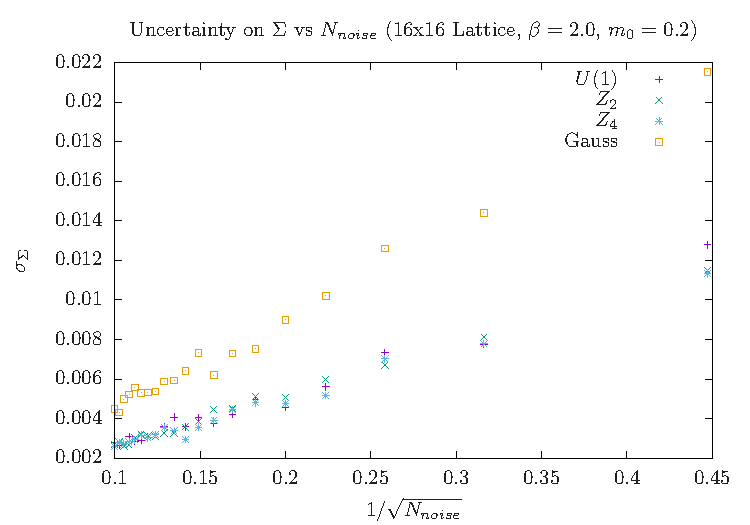
\includegraphics[width=0.8\linewidth]{images/noise_errors.pdf}
    \caption{$\sigma_\Sigma$ vs $1/\sqrt{N_{noise}}$ for each type of noise vector.}
    \label{fig:noise_errors}
\end{figure}
\begin{figure}[H]
    \centering
    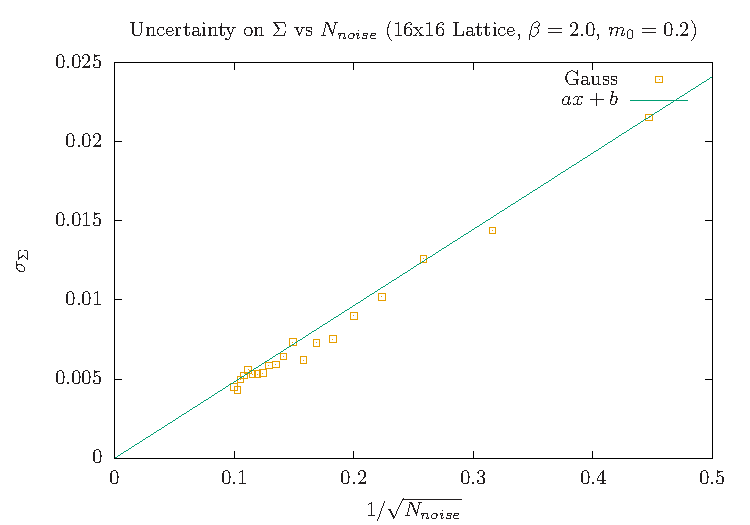
\includegraphics[width=0.8\linewidth]{images/dev_g.pdf}
    \caption{$\sigma_\Sigma$ vs $1/\sqrt{N_{noise}}$ for Gaussian noise vectors.}
    \label{fig:dev_g}
\end{figure}
\begin{figure}[H]
    \centering
    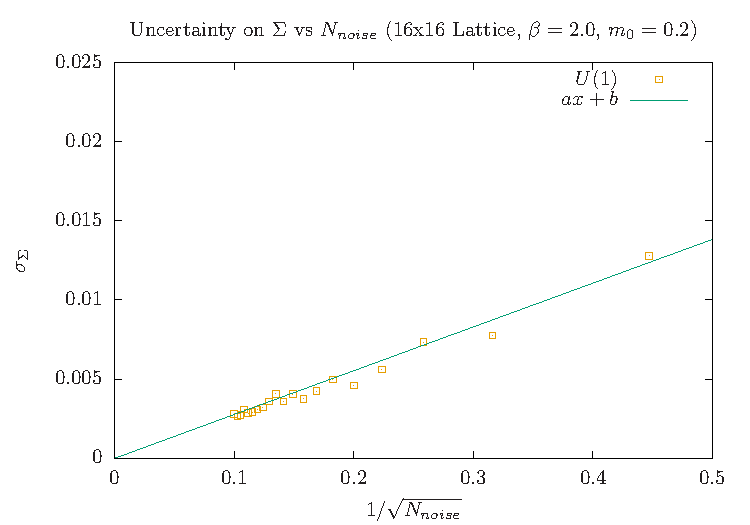
\includegraphics[width=0.8\linewidth]{images/dev_u1.pdf}
    \caption{$\sigma_\Sigma$ vs $1/\sqrt{N_{noise}}$ for $U(1)$ noise vectors.}
    \label{fig:dev_u1}
\end{figure}
\begin{figure}[H]
    \centering
    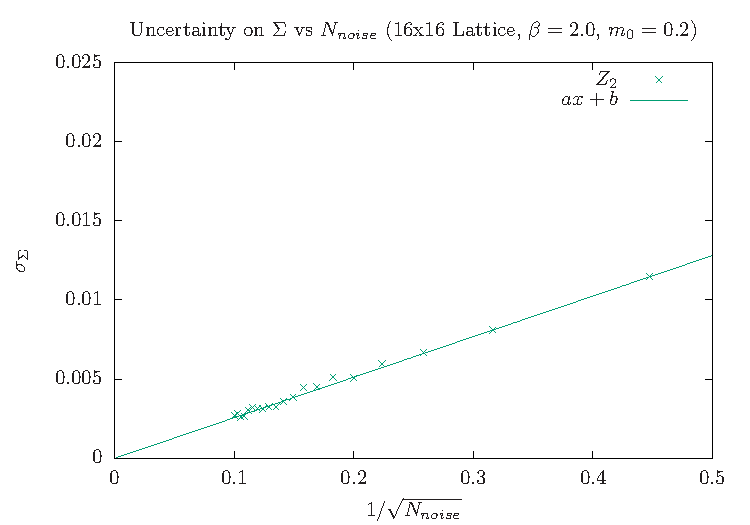
\includegraphics[width=0.8\linewidth]{images/dev_z2.pdf}
    \caption{$\sigma_\Sigma$ vs $1/\sqrt{N_{noise}}$ for $\mathbb{Z}_2$ noise vectors.}
    \label{fig:dev_z2}
\end{figure}
\begin{figure}[H]
    \centering
    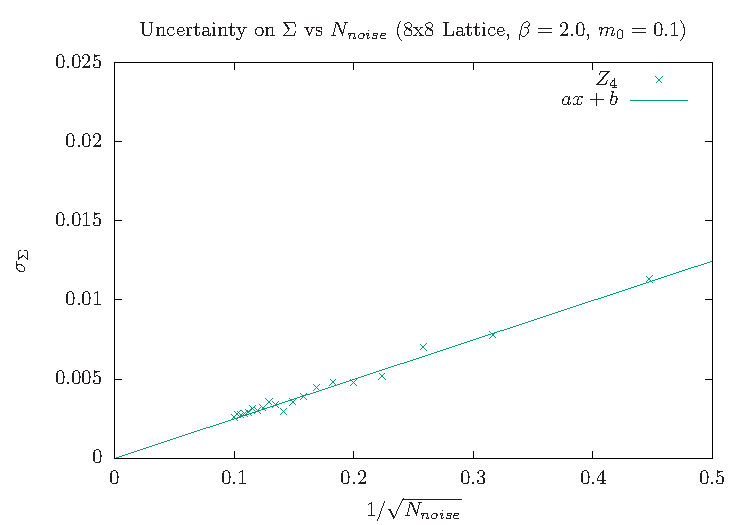
\includegraphics[width=0.8\linewidth]{images/dev_z4.pdf}
    \caption{$\sigma_\Sigma$ vs $1/\sqrt{N_{noise}}$ for $\mathbb{Z}_4$ noise vectors.}
    \label{fig:dev_z4}
\end{figure}
\newpage
\section{Hadron spectroscopy}
After this first analysis regarding some computational techniques applied in lattice computations, we can focus on the low-lying spectrum of our model and its behaviour near the chiral limit. As a first step, we will determine how to define the quark mass $m_f$ in our computations, so that we can drive it to zero in order to approach the chiral limit, where we expect our spectrum to be composed by a massless iso-triplet and a massive iso-singlet state. Consequently, we will proceed with the analysis of the scaling properties of these particles as a function of the fermion mass.
\subsection{Quark mass}
From Noether's theorem, we know that global symmetries of an action are associated with conserved currents. In lattice quantum field theories, given a global transformation of a generic field $\phi(x)$ depending on a continuous parameter $\varepsilon$ connected with the identity:
\begin{equation}
    \phi'_i(x) = \phi_i(x) + i \varepsilon \chi_i (x) 
\end{equation}
where $\chi_i(x)$ is a generic function of the fields in our theory, and the transformation leaves the action invariant:
\begin{equation}
    S[\phi_i] = S'[\phi'_i]
\end{equation}
then there exists a conserved current $J_\mu(x)$ such that, when inserted in a correlation function with an arbitrary operator $\mathcal{O}$, it satisfies:
\begin{equation}
    \langle \partial_\mu J_\mu (x) \mathcal{O}(y) \rangle = \langle \frac{\delta \mathcal{O}(y)}{\delta \phi_i(x)} \chi_i(x) \rangle
\end{equation}
and we say that the current is conserved because if $y \neq x$, then the RHS vanishes and we get an analog of $\partial_\mu J_\mu = 0$.
\\ In a QFT symmetries may be broken spontaneously or due to anomalies, for instance if the integration measure of the path integral is not invariant under the associated transformation. More generally, if the integration measure is preserved by a global transformation, we get operator relations of the form:
\begin{equation}
    \langle \delta \mathcal{O} \rangle - \langle \mathcal{O} \delta S \rangle = 0
\end{equation}
which are called Ward-Takahashi identities \cite{1950PhRv...78..182W, 1957NCim....6..371T}.
\\ The massive 2-flavour Schwinger Model with Wilson fermions is described by the action:
\begin{equation}
     S[U, \psi, \Bar{\psi}] = S_g[U] + S_F[U, \psi, \Bar{\psi}]
\end{equation}
with:
\begin{equation}
\begin{split}
    S_g[U] & = -\beta \sum_{P} \Re{U_P} \\
    S_F[\psi, \Bar{\psi}, U] & = \sum_{\substack{n, m \\ \alpha, \beta}} \Bar{\psi}_\beta(m) D_{\beta, \alpha}(m, n) \psi_\alpha(n) = \\ & = \sum_{n, \alpha} \Bar{\psi}_\alpha(n) \psi_\alpha(n) - \kappa \sum_{n, \mu} \left[ \Bar{\psi}(n)(1 - \gamma_\mu) U_\mu(n) \psi(n+\hat{\mu}) + \right. \\ & \hspace{40mm} \left. + \Bar{\psi}(n)(1 + \gamma_\mu) U_\mu^\dagger (n - \mu) \psi(m - \hat{\mu}) \right]
\end{split}
\end{equation}
The terms in $S_F$ break chiral symmetry explicitly, and the action has only the vectorial $SU(2)_V \times U(1)_V$ global symmetries. The axial $SU(2)_A \times U(1)_A$ symmetries are broken for massive fermions even for the QFT defined in the continuum, where the Ward identity associated with the axial $SU(2)_A$ generators reads:
\begin{equation}\label{continuum PCAC}
    \partial_\mu J^{\mu, a, 2} = 2 m_0 \pi^a
\end{equation}
with the definitions:
\begin{equation}
    \pi^a = \Bar{\psi} \left(\frac{\tau^a \otimes \gamma^{2}}{2}\right) \psi \hspace{10mm} J^{\mu, a, 2} = \Bar{\psi} \left(\frac{\tau^a \otimes \gamma^{\mu} \gamma^{2}}{2}\right) \psi
\end{equation}
where $\tau^a = \sigma^a$ ($a = 1, 2, 3$) are the Pauli matrices acting on flavor space, $\gamma^{\mu}$ ($\mu = 0, 1$= are the continuum equivalent of the Dirac matrices defined in \eqref{gammas}, $\gamma^2 = i\gamma^0\gamma^1$, and $\psi = (u, d)$ is a flavor-doublet.
\\ In \cite{Hip_1998} a lattice equivalent of \eqref{continuum PCAC} was derived to give a definition of the quark mass: using a pseudo-scalar source, we get the lattice PCAC-relation ($x \neq y, \mu = 0, 1$)
\begin{equation}\label{PCAC}
    \sum_\mu \left[ \langle \pi^{a \dagger} (y) J^{a}_{\mu, 2} (x) \rangle - \langle \pi^{a \dagger} (y) J^{a}_{\mu, 2} (x - \hat{\mu}) \rangle \right] = 2m \langle \pi^{a \dagger} (y) \pi^{a} (x) \rangle 
\end{equation}
with the definitions:
\begin{equation}
\begin{split}
   & \pi^a(x) = \Bar{\psi}(x) \left(\frac{\tau^a_{flavor} \otimes \gamma_{2}}{2}\right) \psi(x) \\
   & J^{a}_{\mu, 2}(x) = \frac{1}{2} \left[\Bar{\psi}(x + \hat{\mu}) U^\dagger_\mu(x) \left( \frac{\tau^a_{flavor} \otimes \gamma_\mu \gamma_2}{2} \right) \psi(x) + \Bar{\psi}(x) \left( \frac{\tau^a_{flavor} \otimes \gamma_\mu \gamma_2}{2} \right) U_\mu(x) \psi(x)\right]     
\end{split}
\end{equation}
Notice that in the exact isospin limit, i.e. $m_u = m_d$, the flavor index $a$ is irrelevant, as we get the same relation for each value of $a$, which leads to a mass degenerate iso-triplet of pions. 
\\ By inverting the previous relation, we find that the quark mass $m$ is given by:
\begin{equation}\label{mass}
    m = \frac{1}{2} \frac{\sum_\mu \left[ \langle \pi^{a \dagger} (y) J^{a}_{\mu, 2} (x) \rangle - \langle \pi^{a \dagger} (y) J^{a}_{\mu, 2} (x - \hat{\mu}) \rangle \right]}{\langle \pi^{a \dagger} (y) \pi^{a} (x) \rangle }
\end{equation}
and by computing numerically the RHS with different setups for the bare parameters, we can find the critical fermion coupling $\kappa_c(\beta)$ such that $m$ vanishes.


\subsection{Computation strategy}
Here we will briefly review how to implement the actual computation of the correlation functions mentioned above.
\\ Consider the two-point function for pions. Recall that the correlator $\langle \pi^\dagger(y) \pi(x) \rangle$ consists of a fermionic part $\langle \dots \rangle_F$ where we compute the Grassmann integrals by means of the Wick theorem, and of a gauge part where we take the average of the previous result over all gauge configuration, and so we get an estimate of the hadron propagator.
\\ For instance, if we consider a generic product of operators $C$, the correlation function will be given by:
\begin{equation}
\langle C \rangle = \langle \langle C \rangle_F \rangle_G = \frac{1}{Z} \int \mathcal{D}[U] \, e^{-S_G[U]} \mathcal{D}[\psi, \Bar{\psi}] \, e^{-S_F[{\psi, \Bar{\psi}, U]}} C[\psi, \Bar{\psi}, U]
\end{equation}
and after we carry out the integration over fermionic degrees of freedom, we get:
\begin{equation}
    \langle C \rangle = \frac{1}{Z} \int \mathcal{D}[U] \, e^{-S_G[U]} \det[D]^2 \times (\dots)_F
\end{equation}
with:
\begin{equation}
    Z = \int \mathcal{D}[U]e^{-S_G[U]} \det[D]^2
\end{equation}
where the square factor for the determinants comes from the fact that we are considering two mass-degenerate flavours, and $(\dots)_F$ labels the fermionic contractions coming from the Grassmann integration. We are left with an integral over bosonic degrees of freedom, which can be evaluated through a Monte Carlo simulation as shown in Chapter 2.
\subsubsection*{Pion correlator}
For what concerns the pion correlator, one can show that the result is independent from the flavour index $a$, if we assume exact isospin symmetry (i.e. $D_u$ = $D_d$, since the Dirac operators and propagators for the two flavors would differ only by the value of the mass parameter), and it is given by:
\begin{equation}\label{pion tp}
    \langle \pi^\dagger(y) \pi(x) \rangle = - \frac{1}{2}\tr{\gamma_2 D^{-1}(y, x) \gamma_2 D^{-1}(x, y)} = - \frac{1}{2} \sum_{\alpha, \beta} \abs{D^{-1}(x, y)_{\alpha, \beta}}^2   
\end{equation}
where $\tr(\dots)$ denotes a trace over the spinorial indices $\alpha, \beta$, and in the last step we made use of the $\gamma_2$-hermiticity property of the Dirac propagator:
\begin{equation}
    (\gamma_2)_{\alpha, \alpha'} D^{-1}(x, y)_{\alpha', \beta'}(\gamma_2)_{\beta', \beta} = D^{-1}(y, x)_{\beta, \alpha}^*
\end{equation}
The hadron correlator we are interested in is a combination of matrix elements of the quark propagator, which can be an extremely large matrix with complex entries, hence we need a convenient way to compute it and store it. Each entry $D^{-1}(x,y)_{\alpha, \beta}$ connects a quark with spinorial index $\beta$ defined at a lattice site $y$ (source) to a quark with spinorial index $\alpha$ defined at a lattice site $x$ (sink). These entries in one particular gauge configuration are highly correlated, and consequently we have a reduction of the information content stored in the whole matrix. 
\\ Operatively, one would rather fix a "site" $(\Bar{y}, \Bar{\beta})$ and consider the propagators to all the other sites of the lattice $(x, \alpha)$, which will be stored in one column of the propagator matrix:
\begin{equation}
    D^{-1}(x, \Bar{y})_{\alpha, \Bar{\beta}} = \sum_{y, \beta} D^{-1}(x, y)_{\alpha, \beta} s^{(\Bar{y}, \Bar{\beta})}(y)_{\beta}
\end{equation}
thanks to the introduction of the so-called \textit{point sources}:
\begin{equation}
    s^{(\Bar{y}, \Bar{\beta})}(y)_\beta = \delta(y - \Bar{y}) \delta_{\beta, \Bar{\beta}}
\end{equation}
which are vectors with vanishing components, except for the one associated to the lattice site $\Bar{y}$ and the Dirac index $\Bar{\beta}$, which is fixed to 1.
\\ Since the computation of correlation functions is aimed at the extrapolation of hadron masses, we want to study correlators of hadrons with zero-momentum. %Given a generic hadron interpolator $O(n_x, n_t)$, we can define a state localized on a particular time slice $n_t$ and with definite spatial momentum $p$ by taking the Fourier transform:
%\begin{equation}
%    \Tilde{O}(p, n_t) = \frac{1}{L} \sum_{n_x} O(n_x, n_t) e^{-i a n_x p}
%\end{equation}
Thus we can implement the so-called \textit{wall-to-wall propagators}, where all the points of the time slices associated with the sink and the source contribute to the same correlator:
\begin{equation}\label{C(x0 - y0)}
    C(\abs{x_0 - y_0}) = \frac{1}{L_1} \sum_{x_1, y_1} \langle \pi^\dagger(y_0, y_1) \pi(x_0, x_1) \rangle
\end{equation}
Then we exploit the translational invariance of our system to compute the contributions which concur to correlators with the same time-separation, i.e. we compute the wall-to-wall propagators between all the possible pairs of time slices $(x_0, y_0)$ with the same distance and take the average.
Operatively, this results in fixing a point source in the origin of the lattice, computing the necessary fermionic contraction (i.e. products of $D^{-1}$ matrix elements) and sweeping the fixed source over the whole lattice to repeat the process.


\subsubsection*{Pion-Current}
By means of the Wick theorem, we find that:
\begin{equation}\label{pi-j}
   \begin{split}
     \langle \pi^{a\dagger}(y) J^{a}_{\mu,2}(x) \rangle = & - \frac{1}{2} \Re{U^\dagger_\mu(x) \tr[\gamma_2 D^{-1}(y, x + \hat{\mu}) \gamma_\mu \gamma_2 D^{-1}(x, y)]} = \\
     & = \frac{1}{2} \Re{U^\dagger_\mu(x) \tr[(D^{-1}(x + \hat{\mu}, y))^* \gamma_\mu D^{-1}(x, y)]}
     \\ & = \frac{1}{2} \Re{U^\dagger_\mu(x) \sum_{\alpha, \beta} (D^{-1}(x + \hat{\mu}, y))^*_{\alpha \beta} (\gamma_\mu D^{-1}(x, y))_{\alpha \beta}}
\end{split} 
\end{equation}
The computation strategy is identical to the one embedded for the pion two-point function, but this correlator shows a little additional subtlety: on the RHS of \eqref{pi-j} we find $D^{-1}$ matrix elements defined at different time slices for $\mu = 0$, so we have to take into account the correct anti-periodic boundary conditions in the time direction. Notice also that, since we employ wall-to-wall propagators, the terms coming from $\mu = 1$ on the LHS of \eqref{PCAC} cancel out, and the only non-vanishing contributions come from the term associated to the time derivative.

\subsection{Critical coupling and critical fermion mass}
In order to study the behaviour of the low-lying spectrum of the Schwinger Model, we first need to identify an order parameter which could tell us when the chiral symmetry is expected to be restored. Using the aforementioned PCAC method, we can find the critical fermionic coupling $\kappa_c(\beta)$ at which the quark mass $m_f$ vanishes, so that we know how to approach the chiral limit with our simulations.
\\ In order to study the scaling of the fermion mass, we simulated a $16 \times 16$ lattice for different values of the bare mass $m_0$, with the coupling constant $\beta$ ranging from 1 to 6. Using \eqref{mass} we computed the mass at each possible time separation between sink and source, evaluating typically 2000-5000 configurations and embedding an adequate binning of our data to remove any autocorrelation. Each dataset has been statistically analysed via the jackknife method, so that we could give an estimate of $m_f$ at each time-separation with its error. Figure \ref{fig:mass_plateaus} shows for instance some plots produced for $\beta = 3$ at three different values of $m_0$ (or equivalently, of $\kappa = 1/(2m_0 + 4)$). From each mass plateau, through a fit to a constant, we could extrapolate the value of the quark mass for that system configuration. It is worth to notice that for systems near the chiral limit (e.g. the central mass plateau in (\ref{fig:mass_plateaus})) it has been crucial to consciously gauge the $\varepsilon_{\textrm{MD}}$ parameter which drives the time evolution. Larger values of $\varepsilon_{\textrm{MD}}$ produced indeed low acceptance rates, resulting in stiff gauge configurations, which would prevent us from taking any measurement. 
\begin{figure}[H]
    \centering
    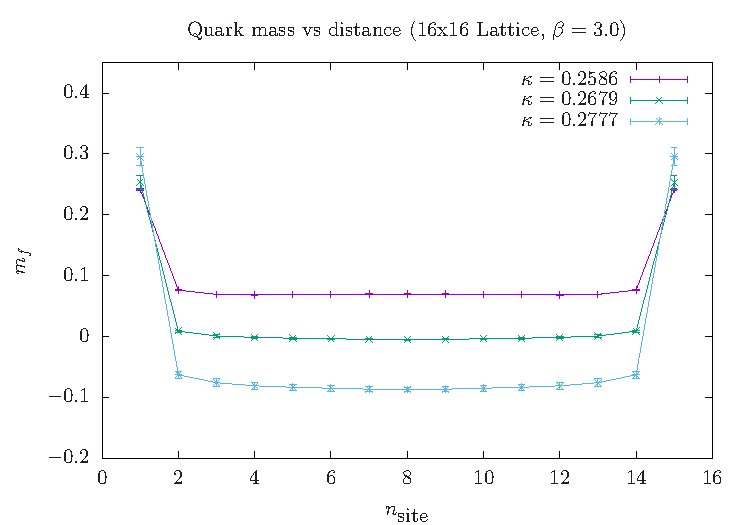
\includegraphics[width=0.7\linewidth]{images/m_corr.pdf}
    \caption{Example of mass plateau computed with \eqref{mass} for $\beta = 3$ at different values of $m_0$ (violet: $m_0 = -0.0667$, green: $m_0 = -0.1333$, blue: $m_0 = -0.2$). The lines have only been added to guide the eye.}
    \label{fig:mass_plateaus}
\end{figure}
Once that we computed $m_f$ for different values of $\kappa(\beta)$, we have been able to extrapolate the critical coupling $\kappa_c$ by performing a linear fit for each value of $\beta$. Figure (\ref{scaling mf}) shows the different measurements and the linear fits, while the estimates of $\kappa_c(\beta)$ are reported in Table \ref{tab:kc} alongside the values of the critical bare mass $m_0^{\textrm{crit}}$. Errors have been estimated from fit and properly propagated in the case of the critical bare mass, for which they are in the order of 1\%. Most measurements show an error bar smaller than the symbol itself.\footnote{Actually, the fit lines should look like filled curves with width $1\sigma$ around the central value, but errors are too small to be visible.}
\begin{figure}
    \centering
    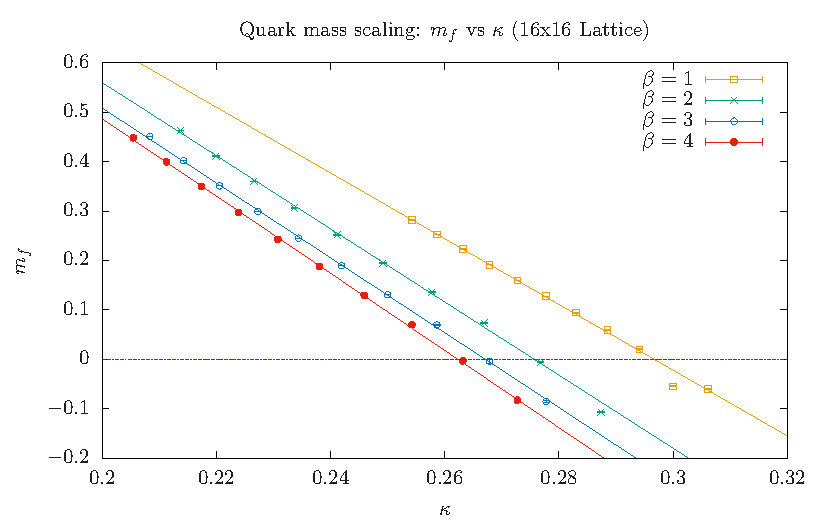
\includegraphics[width=0.8\linewidth]{images/critical.pdf}
    \caption{Scaling of the fermion mass $m_f$ vs $\kappa$ for $\beta = 1, 2, 3, 4$.}
    \label{scaling mf}
\end{figure}
\begin{table}[H]
    \centering
    \begin{tabular}{c|c|c}
      $\beta$ & $\kappa_c$ & $m_0^{\textrm{crit}}$ \\
      \hline \hline 
       1.0  & 0.2967(4) & -0.3148(21) \\
       2.0 & 0.2757(3) & -0.1864(18) \\
       3.0 & 0.2671(2) & -0.1282(10) \\
       4.0 & 0.2623(1) & -0.0939(9) \\
    \end{tabular}
    \caption{Critical coupling $\kappa_c(\beta)$ and $m_0^{\textrm{crit}}$, from fit in (\ref{scaling mf}).}
    \label{tab:kc}
\end{table}

\section{Pseudoscalar Mass}
Through the computation of the pseudoscalar two-point function expressed in Eq. \eqref{pion tp}, one can extrapolate the corresponding hadron mass, and given the similarity with the QCD$_4$ spectrum, in this section we will refer to these particles as \textit{pions} $\pi$.
From the spectral decomposition of Eq. \eqref{C(x0 - y0)}, one can show that at a time separation $n_t$ between sink and source:
\begin{equation}\label{sum spectral}
    C(n_t) = \sum_k \langle 0 | \pi | k \rangle \langle k | \pi^\dagger | 0 \rangle e^{-n_t E_k}
\end{equation}
hence if the interpolators $\pi$ couple to single particle intermediate states, the low-lying energy values $E_k$ will correspond to the hadronic masses we are looking for.
\\ In Figure \eqref{fig:pp} we show some examples of pseudoscalar correlation functions, obtained on $24 \times 24$ lattice with $\beta = 5.0$ and critical coupling $\kappa$ near the critical value. For time separations $n_t$ in the linear regions of the logarithmic plots we expect the sum in \eqref{sum spectral} to be dominated by a single exponential $\sim \exp(-n_t E_0)$, and the contributions coming from higher-energy states can be neglected.
\begin{figure}
    \centering
    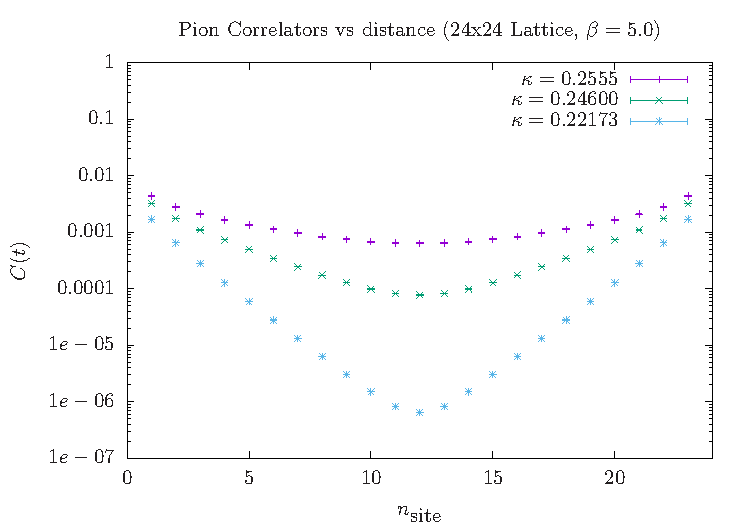
\includegraphics[width=0.7\linewidth]{images/pp.pdf}
    \caption{Pseudoscalar correlation functions at different values of $\kappa$. These are the results of simulations where we processed 4000-5000 gauge configurations.}
    \label{fig:pp}
\end{figure}
In order to extract the pseudoscalar mass $m_{\pi}$, one can define the \textit{effective pseudoscalar mass} as:
\begin{equation}
    m_\pi(n_t + 1/2) = \ln \frac{C(n_t)}{C(n_t + 1)}
\end{equation}
and once the correlator $C(n_t)$ becomes dominated by a single exponential (i.e. the ground state), the effective mass becomes constant and forms a plateau in correspondence of the lowest energy value $E_0$. Anyway, this technique may give problems around $L_0/2$, where $L_0$ is the time-extent of our lattice, therefore it is convenient to exploit the periodicity in $n_t$ of the correlation function. Indeed one can recast the previous expression in the form of:
\begin{equation}\label{meff}
    \frac{C(n_t)}{C(n_t + 1)} = \frac{\cosh(m_\pi(n_t - L_0/2)))}{\cosh(m_\pi (n_t + 1 - L_0/2))}
\end{equation}
and solve numerically for $m_\pi$ at each $n_t$, and this is how we proceeded. Equivalently, one can use:
\begin{equation}\label{meff2}
    m_\pi(n_t) = \textrm{acosh}\left(\frac{C(n_t + 1) + C(n_t - 1)}{2C(n_t)}\right)
\end{equation}
and this relation was used as a double-check on our data.
\\ As we implemented a binning method in the computation of the correlation functions, in order to extract the effective mass with its error we constructed jackknife clusters for the primary variables $C(n_t)$ at each value of $n_t$, and using \eqref{meff} we created jackknife clusters also for the effective masses, then we followed a typical jackknife data analysis. This allowed us to plot the mass plateau for the pseudoscalar correlation functions reported in Figure \eqref{fig:mass plat pions}, and though a fit to a constant we were able to extract $m_\pi$. 
\begin{figure}
    \centering
    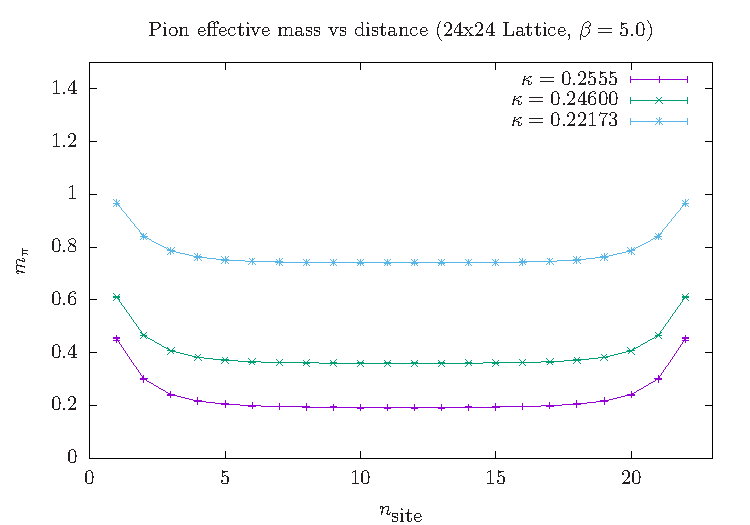
\includegraphics[width=0.7\linewidth]{images/pp_mass.pdf}
    \caption{Mass plateaus for the effective pseudoscalar mass $m_\pi$. These plots refer to the same configurations simulated in \eqref{fig:pp}. The lines were drawn only to guide the eye.}
    \label{fig:mass plat pions}
\end{figure}

\subsection{Finite size corrections}
Before we move on to the analysis of the scaling properties of iso-triplet particles, we need to take into account possible sources of systematic errors in the estimate of the pseudoscalar mass. Lattice simulations may indeed suffer from errors due to the finite size of the simulated system, therefore we need to consider some corrections for the quantities we want to compute. In Ref. \cite{Gutsfeld_1999, Luscher:1986pf} a theoretical and numerical analysis of the asymptotic finite size corrections for the pseudoscalar mass has been carried on for the Schwinger Model.
\\ Given this consideration, we reproduced a study for the scaling properties of $m_\pi$ with respect to the extent of our lattice $L$. In the aforementioned references, it is suggested to correct the pseudoscalar mass estimate accordingly to the following relation:
\begin{equation}\label{rescale}
    m_\pi(L) = m_\pi^{\infty} + A\frac{\sqrt{m_\pi^{\infty}}}{\sqrt{L}}e^{-m_{\pi}^{\infty}L}
\end{equation}
where $m_\pi^{\infty}$ labels the pion mass in the infinite volume limit, while $A$ is a numerical constant.
\begin{figure}
    \centering
    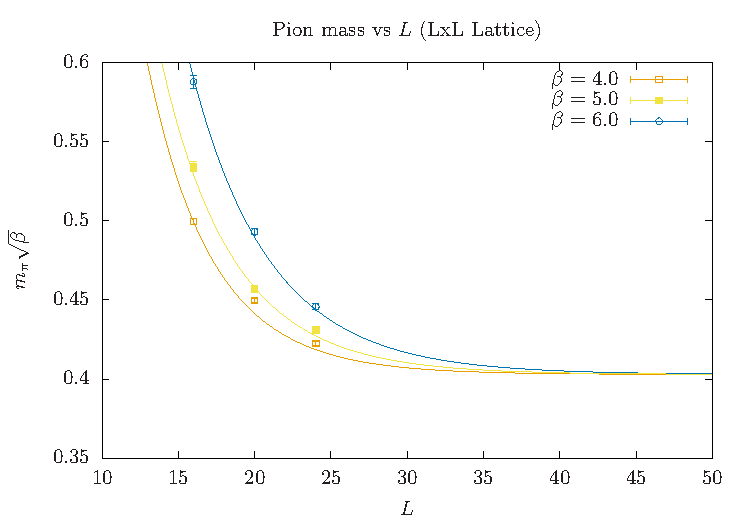
\includegraphics{images/mL.pdf}
    \caption{Scaling of $m_\pi \sqrt{\beta}$ against $L$. We plotted the values collected at $\beta = 4, 5, 6$ for $z = (m_f \sqrt{\beta})^{2/3} = 0.2$. We used three different values of $L = 16, 20, 24$. The solid lines represent fit curves obtained through Eq. \eqref{rescale}.}
    \label{fig: m vs L}
\end{figure}
In Figure \eqref{fig: m vs L} we plot the relation in Eq. \eqref{rescale} rescaled by $\sqrt{\beta}$ for various values of $\beta$. Unfortunately, we only had three available values of $L$, and a broader dataset would have helped to test the finite size effects more consistently. Anyway, our results seem to be in accordance with the aforementioned relation, and from a fit of the curves for $\beta = 4, 5, 6$ we gave an universal estimate for $A = 10.2(2)$.
\\ The measurements reported in Figure \eqref{fig: m vs L} were taken at a fixed value of the scaling parameter $z = (m_f \sqrt{\beta})^{2/3} = 0.2$, where $m_f$ is the quark mass estimated from the PCAC relation. 

\subsection{Scaling of the pseudoscalar mass}
Before we show the numerical results of our simulations, it is interesting to see some approximate calculations for $m_\pi \sqrt{\beta}$ for the massive Schwinger Model in the continuum. The first calculation was performed by Smilga in \cite{PhysRevD.55.R443}, where from a classical analysis it follows that for strong coupling and small fermion mass:
\begin{equation}\label{Smilga}
    m_\pi^{\textrm{cont}}\sqrt{\beta} \simeq 2^{5/6} e^{\gamma/3} \left(\frac{\Gamma(3/4)}{\Gamma(1/4)}\right)^{2/3} \frac{\Gamma(1/6)}{\Gamma(2/3)} (m_f \sqrt{\beta})^{2/3} = 2.008\dots (m_f \sqrt{\beta})^{2/3}
\end{equation}
where $e$ is the coupling constant of the theory, while $\gamma$ is the Eulero-Maschironi constant.
\\ On the other hand, for large masses a semi-classical analysis was performed by Gattringer in Ref. \cite{https://doi.org/10.48550/arxiv.hep-th/9503137}, where the following relation was found:
\begin{equation}\label{Gatt Cont}
     m_\pi^{\textrm{cont}}\sqrt{\beta} \simeq e^{2\gamma/3} \frac{2^{5/6}}{\pi^{1/6}} \left(m_f \sqrt{\beta}\right)^{2/3} = 2.163\dots(m_f \sqrt{\beta})^{2/3}
\end{equation}
and we can compare our non-perturbative results with this predictions.
\begin{table}
    \centering
    \begin{tabular}{c|c|c|c}
        $z$ & $\beta$ & $m_0$ & $m_{\pi}^{\infty}\sqrt{\beta}$  \\
        \hline \hline
        0.2 & 1.0 & -0.231367 & 0.398(1) \\
        0.2 & 2.0 & -0.132316 & 0.415(2) \\
        0.2 & 3.0 & -0.082626 & 0.419(3) \\
        0.2 & 4.0 & -0.057374 & 0.417(5) \\
        0.2 & 5.0 & -0.043199 & 0.425(23) \\
        0.2 & 6.0 & -0.034249 & 0.431(19) \\
        0.4 & 1.0 & -0.075308 & 0.745(1) \\
        0.4 & 2.0 & -0.017495 & 0.792(1) \\
        0.4 & 3.0 & 0.014505 & 0.805(1) \\
        0.4 & 4.0 & 0.026358 & 0.809(2) \\
        0.4 & 5.0 & 0.032526 & 0.817(3) \\
        0.4 & 6.0 & 0.036146 & 0.824(2) \\
        0.8 & 1.0 & 0.352443 & 1.357(1) \\
        0.8 & 2.0 & 0.314017 & 1.528(1) \\
        0.8 & 3.0 & 0.298677 & 1.607(1) \\
        0.8 & 4.0 & 0.276568 & 1.640(2) \\
        0.8 & 5.0 & 0.255009 & 1.653(1) \\
        0.8 & 6.0 & 0.239625 & 1.688(2) \\
    \end{tabular}
    \caption{Extrapolation of the pseudoscalar mass for a $16 \times 16$ lattice. To fix the scaling parameter $z = (m_f \sqrt{\beta})^{2/3}$, we used the suggested values of $m_0$ reported in \cite{Christian_2006} and checked using the PCAC relation. Typical statistics of the runs were 4000-5000 configurations.}
    \label{tab: pion 16}
\end{table}
\begin{table}
    \centering
    \begin{tabular}{c|c|c|c}
        $z$ & $\beta$ & $m_0$ & $m_{\pi}^{\infty}\sqrt{\beta}$  \\
        \hline \hline
        0.2 & 1.0 & -0.231367 & 0.389(1) \\
        0.2 & 2.0 & -0.132316 & 0.415(1) \\
        0.2 & 3.0 & -0.082626 & 0.420(1) \\
        0.2 & 4.0 & -0.057374 & 0.417(2) \\
        0.2 & 5.0 & -0.043199 & 0.394(3) \\
        0.2 & 6.0 & -0.034249 & 0.416(4) \\
        0.4 & 1.0 & -0.075308 & 0.746(4) \\
        0.4 & 2.0 & -0.017495 & 0.788(1) \\
        0.4 & 3.0 & 0.014505 & 0.803(1) \\
        0.4 & 4.0 & 0.026358 & 0.805(1) \\
        0.4 & 5.0 & 0.032526 & 0.816(2) \\
        0.4 & 6.0 & 0.036146 & 0.804(2) \\
        0.8 & 1.0 & 0.352443 & 1.356(1) \\
        0.8 & 2.0 & 0.314017 & 1.528(1) \\
        0.8 & 3.0 & 0.298677 & 1.602(1) \\
        0.8 & 4.0 & 0.276568 & 1.641(1) \\
        0.8 & 5.0 & 0.255009 & 1.657(1) \\
        0.8 & 6.0 & 0.239625 & 1.686(2) \\
    \end{tabular}
    \caption{Extrapolation of the pseudoscalar mass for a $20 \times 20$ lattice.}
    \label{tab: pion 20}
\end{table}
\begin{table}
    \centering
    \begin{tabular}{c|c|c|c}
        $z$ & $\beta$ & $m_0$ & $m_{\pi}^{\infty}\sqrt{\beta}$  \\
        \hline \hline
        0.2 & 1.0 & -0.231367 & 0.385(1) \\
        0.2 & 2.0 & -0.132316 & 0.407(1) \\
        0.2 & 3.0 & -0.082626 & 0.408(1) \\
        0.2 & 4.0 & -0.057374 & 0.409(2) \\
        0.2 & 5.0 & -0.043199 & 0.406(2) \\
        0.2 & 6.0 & -0.034249 & 0.407(3) \\
        0.4 & 1.0 & -0.075308 & 0.745(4) \\
        0.4 & 2.0 & -0.017495 & 0.787(1) \\
        0.4 & 3.0 & 0.014505 & 0.801(1) \\
        0.4 & 4.0 & 0.026358 & 0.805(1) \\
        0.4 & 5.0 & 0.032526 & 0.808(1) \\
        0.4 & 6.0 & 0.036146 & 0.808(1) \\
        0.8 & 1.0 & 0.352443 & 1.357(1) \\
        0.8 & 2.0 & 0.314017 & 1.527(1) \\
        0.8 & 3.0 & 0.298677 & 1.604(1) \\
        0.8 & 4.0 & 0.276568 & 1.642(1) \\
        0.8 & 5.0 & 0.255009 & 1.660(1) \\
        0.8 & 6.0 & 0.239625 & 1.679(1) \\
    \end{tabular}
    \caption{Extrapolation of the pseudoscalar mass for a $24 \times 24$ lattice.}
    \label{tab: pion 24}
\end{table}
\\ We collected values of the pseudoscalar mass for lattices of different size, namely with $L = 16, 20, 24$. The dynamical parameters have been set accordingly to the dataset produced in Ref. \cite{Christian_2006}, so that we could make a comparison of our results. Each measurement of the pseudoscalar mass has been corrected to the infinite volume value accordingly to Eq. \eqref{rescale}, and the results have been reported in Table \eqref{tab: pion 16}, Table \eqref{tab: pion 20} and Table \eqref{tab: pion 24}.
\\ We can draw the conclusion that at any value of the scaling parameter $z$, our measurements of $m_\pi^{\infty}\sqrt{\beta}$ are in good accordance with the reference results for the largest lattice, while for $L = 16$ and $L = 20$ there are more fluctuations at lower values of $z$.
\\ This may come from the fact that the spectral decomposition in \eqref{sum spectral} is dominated by the lightest state only at large distances, and clearly broader lattices allow us to explore bigger time-separations between the pseudoscalar interpolators.
\\ Nonetheless, we still were able to draw some conclusions regarding the continuum predictions mentioned before. In Figure \eqref{fig: beta z02}, \eqref{fig: beta z04} and \eqref{fig: beta z08} we plotted the scaling of $m_\pi^{\infty}\sqrt{\beta}$ against $\beta$ for $z = 0.2, 0.4$ and $0.8$, respectively, and in each plot we also draw with dashed lines the continuum predictions \eqref{Smilga} and \eqref{Gatt Cont}. 
\\ We expect the pseudoscalar mass to reach one of those values for larger $\beta$, since this parameter is linked to the lattice spacing by the relation $\beta = 1/a^2e^2$. For $z = 0.2$, we have that at larger values of $\beta$ the fermion mass becomes sufficiently small, hence we expect the pseudoscalar mass to be near the Smilga prediction \eqref{Smilga}. This behaviour is confirmed for $L = 24$, while the other datasets show large fluctuations and it is not possible to draw a definite conclusion.
\begin{figure}
    \centering
    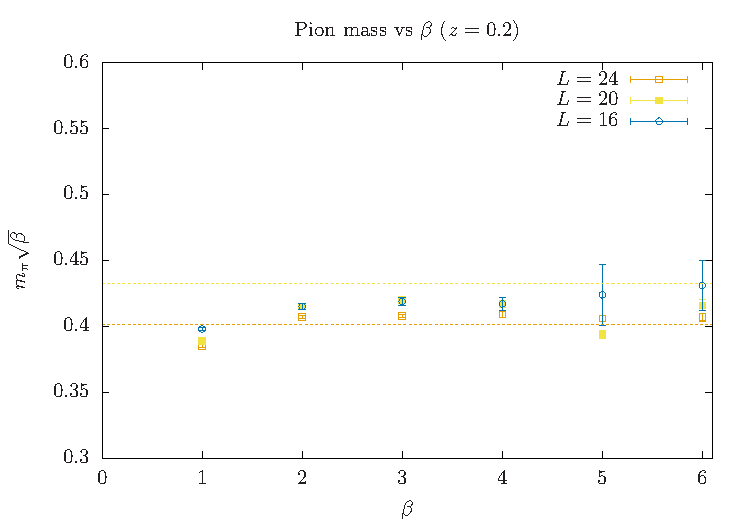
\includegraphics[width=0.8\linewidth]{images/beta02.pdf}
    \caption{Scaling of $m_\pi^{\infty}\sqrt{\beta}$ vs $\beta$ for $z = (m_f \sqrt{\beta})^{2/3} = 0.2$. Upper dashed line: continuum prediction \eqref{Smilga}, lower dashed line: continuum prediction \eqref{Gatt Cont}.}
    \label{fig: beta z02}
\end{figure}
\\ For $z = 0.4$ we have a similar outcome, and indeed the plots with $L = 24$ and $L = 20$ clearly show a drift in the scaling curves towards the classical prediction by Smilga. For $z = 0.8$ the scaling behaviour changes: the fermion mass is now further from the chiral limit, hence all the datasets seem to tend toward the semi-classical prediction \eqref{Gatt Cont}. 
\begin{figure}
    \centering
    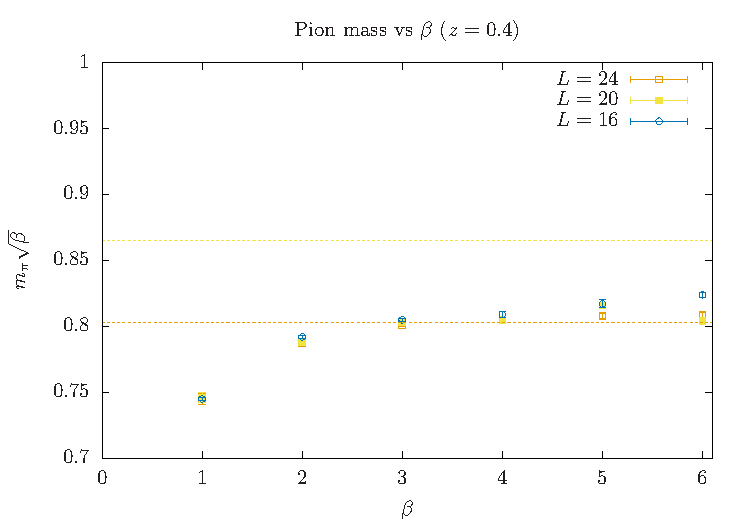
\includegraphics[width=0.8\linewidth]{images/beta04.pdf}
    \caption{Scaling of $m_\pi^{\infty}\sqrt{\beta}$ vs $\beta$ for $z = (m_f \sqrt{\beta})^{2/3} = 0.4$}
    \label{fig: beta z04}
\end{figure}
\begin{figure}
    \centering
    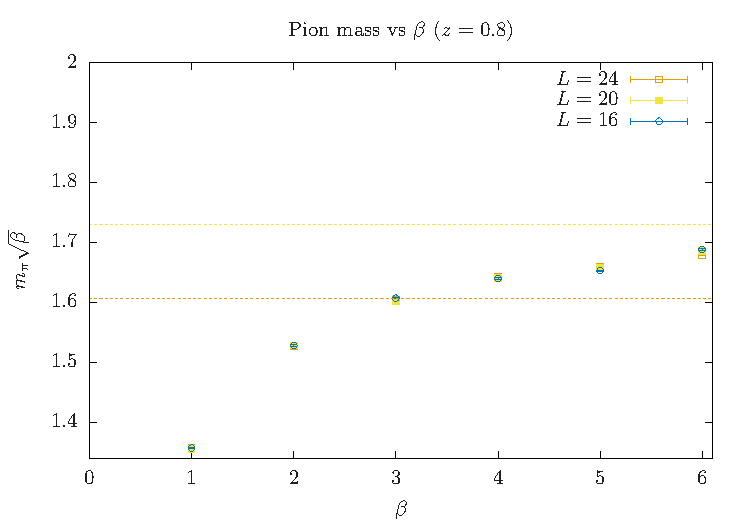
\includegraphics[width=0.8\linewidth]{images/beta08.pdf}
    \caption{Scaling of $m_\pi^{\infty}\sqrt{\beta}$ vs $\beta$ for $z = (m_f \sqrt{\beta})^{2/3} = 0.8$}
    \label{fig: beta z08}
\end{figure}
\newpage
As a final study, we can now check the scaling properties of the pseudoscalar mass with respect to the parameter $z$, in particular for what concerns its behaviour towards the chiral limit. In Figure \eqref{fig: scaling z} we report the result obtained on a $20 \times 20$ lattice for $\beta = 2$ and $4$.
The values of the quark mass $m_f$ have been computed with the PCAC relation as usual, and we did not report error bars on it as they were essentially negligible.
All the analysed pseudoscalar masses have been corrected to the infinite volume value $m_\pi^\infty$ analogously to what we did before.
\begin{figure}
    \centering
    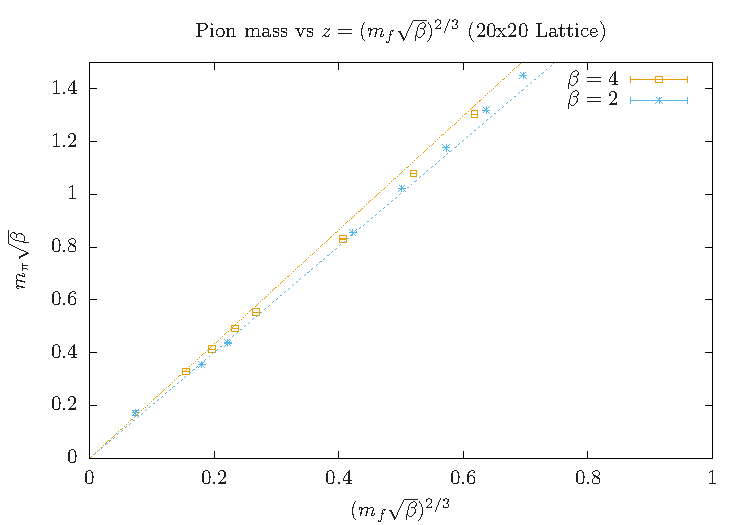
\includegraphics{images/scaling.pdf}
    \caption{Scaling of the pseudoscalar mass $m_\pi^\infty \sqrt{\beta}$ against $z$ for $\beta = 2, 4$. Upper dashed line: semi-classical continuum approximation \eqref{Gatt Cont}, lower dashed line: classical continuum approximation \eqref{Smilga}. We collected each measure studying 10000 configurations.}
    \label{fig: scaling z}
\end{figure}
The dashed lines in the plot are the continuum approximations previously defined, and the measurements seem to be coherent with these predictions. For larger values of $z$, we have higher values of the fermion mass, and $m_\pi^\infty\sqrt{\beta}$ drifts slightly more towards the semi-classical approximation. To draw more precise conclusion regarding the accordance with these relations towards the chiral limit, it would have been necessary to collect more data at lower values of $z$, but the results for $\beta = 2$ seem to be in very good accordance with the classical analytical result.
Altogether it is clear that the pseudoscalar mass tends to zero as the fermion mass vanishes, hence the approach to the chiral limit respects our prediction.
\newpage
\section{Iso-singlet state}
Now we can focus on the behaviour of the iso-singlet state, which we can call an "$\eta$-meson" in analogy with QCD$_4$. This state does not carry any flavor-index and its spinorial structure is given by:
\begin{equation}
    \eta(x) = \frac{1}{2} \Bar{\psi}(x) \left(\mathbb{1}_{flavor} \otimes \gamma_2\right) \psi(x)
\end{equation}
where as usual $\psi = (u, d)$ is a flavor-doublet and $\gamma_2 = i \gamma_0 \gamma_1$. We are interested in the computation of its two-point function $\langle \eta^\dagger(y) \eta(x) \rangle$, which takes contributions from the so-called \textit{disconnected pieces}, and these expressions require an higher computational effort with respect to the connected terms we encountered for the pion correlation function. Namely, using the Wick theorem to compute the fermionic contractions we find that:
\begin{equation}
\begin{split}
        \langle \eta^\dagger(y) \eta(x) \rangle &= \langle \tr[\gamma_2 D^{-1}(y,y)]\tr[\gamma_2 D^{-1}(x,x)] - \frac{1}{2}\tr[\gamma_2 D^{-1}(y,x) \gamma_2 D^{-1}(x,y)] \rangle \\
        &= \langle \tr[\gamma_2 D^{-1}(y,y)]\tr[\gamma_2 D^{-1}(x,x)]\rangle -\frac{1}{2} \sum_{\alpha, \beta} \abs{D^{-1}_{\alpha, \beta}(x,y)}^2
\end{split}
\end{equation}
where the second term corresponds to the pion two-point function \eqref{pion tp}, while the first term corresponds to the disconnected contributions, which are given by the combination of propagators matrix elements of the form $D^{-1}(x,x)_{\alpha, \beta}$, i.e. propagators which transport a fermion from a site $x$ back to the same site.
\\ The computation strategy for these terms is still based on the introduction of point sources, analogously to what we did for the iso-triplet states, but the computational resources needed to store all the necessary contributions are way higher. Operatively, this was sensibly visible from the fact that simulations which endowed this computation were much longer and produced results with less accuracy, given the same statistics volume.
\\ Consider for instance Figure \eqref{fig: eta corr}, which shows the correlation function of the iso-singlet state computed on a $20 \times 20$ lattice ($\beta = 2$, $\kappa = 0.21367$), and compare it with the analogous plots for the iso-triplet states \eqref{fig:pp}. The linear behaviour (on a logarithmic scale), where we expect the spectral decomposition to be dominated by a single state, is still clearly visible, but the values towards the central region are affected by large errors.
\begin{figure} 
    \centering
    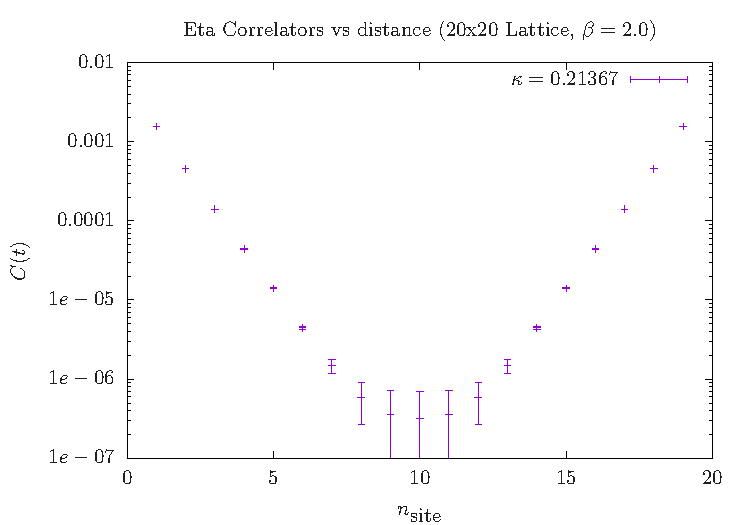
\includegraphics[width = 0.8\linewidth]{images/eta_corr.pdf}
    \caption{Correlation function for the $\eta$-meson, computed for $\beta = 2$ and $\kappa = 0.21367$. In these runs we processed 5000 gauge configurations.}
    \label{fig: eta corr}
\end{figure}
The statistical uncertainty of our measurements and the higher computational effort required to process these simulations prevented us from performing a deeper analysis for this state, similarly to what we did for the pseudoscalar mass, hence we analysed the scaling properties of the $\eta$-meson mass exploiting the results found for $m_\pi$. 

\subsection{Scaling of $m_\eta$}
The computation of $m_\eta$ was performed following the same procedure as for the pseudoscalar mass $m_\pi$, namely extrapolating the effective mass numerically with Eq. \eqref{meff} and correcting the result with the infinite volume extrapolation \eqref{rescale}.
\\ The iso-singlet state remains massive in the chiral limit, and from a semi-classical analysis it was found that for the continuum Schwinger Model $m_\eta$ is described by the relation:
\begin{equation}\label{prediction eta}
    m_\eta \sqrt{\beta} = \sqrt{\frac{2}{\pi} + \left(m_\pi \sqrt{\beta}\right)^2}
\end{equation}
hence when we reach the chiral limit and the pion mass vanishes, the mass $m_\eta$ approaches the value:
\begin{equation}
    m_\eta \sqrt{\beta} = \sqrt{\frac{2}{\pi}}
\end{equation}
In Figure \eqref{fig: scaling eta} we reported the analysis of the scaling properties of $m_\eta^{\infty}\sqrt{\beta}$ performed on a $20 \times 20$ lattice for $\beta = 2$ and $4$. The fermion mass was newly found through the PCAC relation, so that we could estimate the scaling parameter $z = (m_f \sqrt{\beta})^{2/3}$. 
\\ The dashed lines in the plot correspond to the theoretical prediction \eqref{prediction eta}, where we used the approximations \eqref{Smilga} (lower line) and \eqref{Gatt Cont} (upper line) as an input for the pion mass. The horizontal line represents the expected value for $m_\eta \sqrt{\beta}$ in the chiral limit. The correct behaviour is more evident for $\beta = 4$, since we are closer to the continuum limit, but better conclusion could be drawn by collecting more data at lower values of $z$, given the large errors and fluctuations which affect our measurements in this region.
\begin{figure}
    \centering
    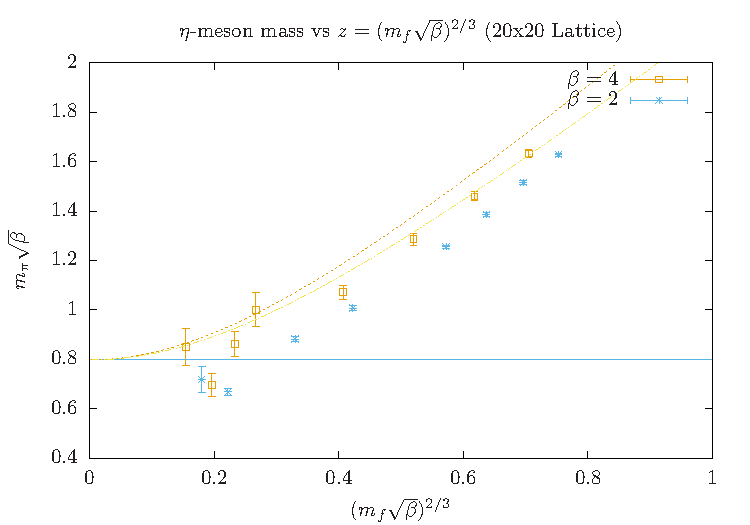
\includegraphics{images/scaling_eta.pdf}
    \caption{Scaling of $m_\eta^\infty\sqrt{\beta}$ as a function of $z = (m_f \sqrt{\beta})^{2/3}$. Upper dashed line: theoretical prediction \eqref{prediction eta} with the insertion of the semi-classical approximation \eqref{Gatt Cont} for $m_\pi\sqrt{\beta}$. Lower dashed line: theoretical prediction with the insertion of the classical approximation \eqref{Smilga}. We collected each measure studying 10000 configurations.}
    \label{fig: scaling eta}
\end{figure}
For what concerns the analytical prediction \eqref{prediction eta}, the relation describes moderately well our data for $\beta = 4$, in particular when we input Smilga's classical prediction for the pion mass. Typically, the behaviour predicted by this semi-classical analysis would be more evident at larger values of the fermion mass $m_f$, while at smaller values the quantum fluctuations become more significant, resulting in a larger deviation from the analytical formula.
\\ In conclusion, the analysis for the iso-singlet state cannot be accounted as completely satisfying, but its general behaviour towards the chiral limit seems to be reasonably described, i.e. the $\eta$-meson remains massive when the fermion mass vanishes, and its value tends to $\sqrt{2/\pi}$.